\chapter{相关理论与技术}

\section{引言}

本章对后续章节所用到的相关理论和技术进行简单阐述,主要包括常用的聚类算法(k-means算法和k-medoids算法)以及聚类算法的评估标准、稀疏矩阵的存储方式和多项式拟合技术,最后简单介绍了马尔科夫链模型。这些理论为后续研究提供了理论基础。

\section{聚类算法}
聚类算法是一种无监督学习算法,数据集中的每个数据项不带有标签信息,通过统计分析技术将数据集分成不同的子集或簇,使得分到同一子集或簇的成员对象都有某种相似的特征。这种技术被广泛应用于各个领域,包括机器学习、数据挖掘、模式识别等。

\subsection{k-means算法}

k-means算法由文献\cite{hartigan1979algorithm}正式提出,现已成为数据挖掘中常用的聚类算法,其算法主要思路是一种启发性算法,求解过程利用了EM算法\citing{AMaximum},通过不断迭代优化直到满足停止迭代的条件。

\subsubsection{算法流程及复杂度分析}

现有样本集$D=\left\{x_1,x_2,...,x_m\right\}$,k-means算法将数据集划分成互不相交的K个簇$C=\left\{C_1,C_2,...,C_K\right\}$,且满足$C_1\bigcup{C_2\bigcup{...\bigcup{C_m=D}}}$,每个簇的簇心$\mu _i=\frac{1}{|C_i|}\sum_{\mathbf{x}\in C_i}{\mathbf{x}}$。
算法流程如下:\\
\begin{algorithm}[H]
	 \KwData{样本集$D=\left\{x_1,x_2,...,x_m\right\}$,簇个数K}
	 \KwResult{簇划分$C=\left\{C_1,C_2,...,C_k\right\}$}
	 从数据集D中随机初始化K个样本,将其作为K个初始簇心\;
	 \Repeat{所有簇心不再更新或更新值小于一定阈值}{
		 将所有的簇置为空,$C_i=\varPhi \,\,\left( 1\leqslant i\leqslant K \right)$\;
		 \For{i=1,2,...,m}{
		 	计算样本$x_i$与所有簇心之间的距离,并将$x_i$归为第$\alpha _i$类,使其满足:\\
		 	$\alpha _i=arg\,\,\min \left( d_{i\alpha _i} \right) $\\其中:
		 	$d_{i\alpha _i}=||x_i-\mu _{\alpha _i}||_2$\;
		 	将样本$x_i$划入簇$C_{\alpha _i}$\;
		 }
		 \For{i=1,2,...,K}{
		 	$\hat{\mu}_i=\frac{1}{|C_i|}\sum_{x\in C_i}{x}$\;
		 	\If{$\hat{\mu}_i\ne \mu _i$}{
		 		$\mu _i$=$\hat{\mu}_i$\;
		 	}
		 }
	 }
	 \caption{k-means算法}
	\label{kmeans}
\end{algorithm}

从上述流程可以得到,k-means算法复杂度为O(n*k*t),其中n表示样本数目,k表示簇个数,t是平均迭代次数。k-meas算法的收敛性可参考论文\cite{neal1998view}。

\subsection{k-medoids算法}
k-means算法要求所有元素维度相同且距离度量必须基于欧式距离,如果需要对不规整的数据进行聚类,k-means算法显然无法解决此类聚类问题。针对不规整的数据,可以采用k-medoids算法\citing{rdusseeun1987clustering}进行聚类。k-medoids算法只需输入距离矩阵即可,所以对距离度量方法也更加宽泛。k-medoids流程如下:\\
\begin{algorithm}[H]
	 \KwData{样本距离矩阵$M_{nn}$,簇个数K}
	 \KwResult{簇划分$C=\left\{C_1,C_2,...,C_k\right\}$}
	 随机初始化K个样本,将其对应的序号作为K个初始簇心\;
	 \Repeat{所有簇心不再更新或更新值小于一定阈值}{
		 将所有的簇置为空,$C_i=\varPhi \,\,\left( 1\leqslant i\leqslant K \right)$\;
		 \For{i=1,2,...,m}{
		 	依据距离矩阵,计算序号为i的样本与所有簇心之间的距离,并将序号为i的样本归为第$\alpha _i$类,使其满足:\\
		 	$\alpha _i=arg\,\,\min \left( M[i\,\mu_{\alpha _i}] \right) $\;
		 }
		 \For{i=1,2,...,K}{
		 	$\hat{\mu }_i=arg\,\,\min_{x\in C_i} \left( \sum_{j\in C_i}{M\left[ x,j \right]} \right) $\;
		 	\If{$\hat{\mu}_i\ne \mu _i$}{
		 		$\mu _i$=$\hat{\mu}_i$\;
		 	}
		 }
	 }
	 \caption{k-medoids算法}
\end{algorithm}

从上述流程可以得到,k-medoids算法复杂度同k-means一样为O(n*k*t),其中n表示样本数目,k表示簇个数,t是平均迭代次数。


\subsection{聚类评估指标}
聚类评估指标可以分为两种\citing{zhouzh2016},
一类是将聚类结果与某个“参考模型”进行比较,度量这种比较结果的评估指标称为“外部指标”;另一种不依赖标签数据,针对聚类计算后簇内与簇间的距离度量得到的评价指标,称之为“内部指标”。

\subsubsection{外部指标}
假设通过聚类算法将数据集D划分成簇集$C=\left\{C_1,C_2,...,C_K\}\right\}$,参考模型将数据集D划分的簇集$C^*=\left\{ C_{1}^{*},C_{2}^{*},...,C_{K}^{*} \right\} $,相应地,令$\lambda$和$\lambda^{*}$分别表示与C和$C^{*}$对应的簇标记。我们将样本两两配对,定义:
\begin{equation}
\label{abcd}
\begin{aligned}
&a=|S S|, \quad S S=\left\{(x_{i}, x_{j}) | \lambda_{i}=\lambda_{j}, \lambda_{i}^{*}=\lambda_{j}^{*}, i<j)\right.\\
&b=|S D|, \quad S D=\left\{(\boldsymbol{x}_{i}, \boldsymbol{x}_{j}) | \lambda_{i}=\lambda_{j}, \lambda_{i}^{*} \neq \lambda_{j}^{*}, i<j)\right.\\
&c=|D S|, \quad D S=\left\{(\boldsymbol{x}_{i}, \boldsymbol{x}_{j}) | \lambda_{i} \neq \lambda_{j}, \lambda_{i}^{*}=\lambda_{j}^{*}, i<j)\right.\\
&d=|D D|, \quad D D=\left\{(\boldsymbol{x}_{i}, \boldsymbol{x}_{j}) | \lambda_{i} \neq \lambda_{j}, \lambda_{i}^{*} \neq \lambda_{j}^{*}, i<j)\right.
\end{aligned}
\end{equation}

其中集合SS包含了在C中和在$C^{*}$中隶属于同一簇的样本对,集合SD包含了在C中隶属于相同簇但在$C^{*}$中隶属于不同簇的样本对,......因为任意一个样本对$\left(\boldsymbol{x}_{i}, \boldsymbol{x}_{j}\right)(i<j)$均只能隶属于其中一个集合,因此有$a+b+c+d=m(m-1) / 2$成立。

基于\ref{abcd},可引出Rand指数的定义:
\begin{equation}
\label{RI}
\mathrm{RI}=\frac{2(a+d)}{m(m-1)}
\end{equation}

RI指数取值范围为[0,1],其值越大表示聚类效果越好,反之,则聚类效果越差。

但是Rand指数对于不同聚类结果的区分度不高,于是基于Rand指数,提出了Adjusted Rand Index\citing{rand1971objective}。
\[
\begin{array}{c|ccccc}
	&		C_{1}^{*}&		C_{2}^{*}&		\dots&		C_{S}^{*}&		\,\,\text{Sums}\\
	\hline
	C_1&		n_{11}&		n_{12}&		\dots&		n_{1S}&		a_1\\
	C_2&		n_{21}&		n_{22}&		\dots&		n_{2S}&		a_2\\
	\vdots&		\vdots&		\vdots&		\ddots&		\vdots&		\vdots\\
	C_K&		n_{K1}&		n_{K2}&		\cdots&		n_{KS}&		a_K\\
	\,\,\text{Sums}&		b_1&		b_2&		\dots&		b_S&		\\
\end{array}
\]

其中$n_{ij}$表示簇$C_{i}$和簇$C_{i}^{*}$之间共同存在的对象个数,即$n_{i j}=\left|X_{i} \cap Y_{j}\right|$。ARI指数定义如下:
\begin{equation}
\label{ARI}
ARI=\frac{\sum_{ij}{\left( \begin{array}{c}
	n_{ij}\\
	2\\
\end{array} \right)}-\left[ \sum_i{\left( \begin{array}{c}
	a_i\\
	2\\
\end{array} \right)}\sum_j{\left( \begin{array}{c}
	b_j\\
	2\\
\end{array} \right)} \right] /\left( \begin{array}{c}
	n\\
	2\\
\end{array} \right)}{\frac{1}{2}\left[ \sum_i{\left( \begin{array}{c}
	a_i\\
	2\\
\end{array} \right)}+\sum_j{\left( \begin{array}{c}
	b_j\\
	2\\
\end{array} \right)} \right] -\left[ \sum_i{\left( \begin{array}{c}
	a_i\\
	2\\
\end{array} \right)}\sum_j{\left( \begin{array}{c}
	b_j\\
	2\\
\end{array} \right)} \right] /\left( \begin{array}{c}
	n\\
	2\\
\end{array} \right)}
\end{equation}

\subsubsection{内部指标}

若直接评估聚类结果本身,则需要考虑内部指标,同样设定聚类算法得到的簇划分为$C=\left\{C_1,C_2,...,C_K\right\}$。在定义内部指标之前,先定义几种距离公式:
\begin{equation}
\label{distance}
\begin{aligned}
avg(C) &=\frac{2}{|C|(|C|-1)} \sum_{1 \leqslant i<j \leqslant|C|} dist\left(x_{i}, x_{j}\right) \\
diam(C) &=\max _{1 \leqslant i<j \leqslant|C|} dist\left(x_{i}, x_{j}\right) \\
d_{\min }\left(C_{i}, C_{j}\right) &=\min _{x_{i} \in C_{i}, x_{j} \in C_{j}} dist\left(x_{i}, x_{j}\right) \\
d_{cen}\left(C_{i}, C_{j}\right) &=dist\left(\mu_{i}, \mu_{j}\right)
\end{aligned}
\end{equation}

其中,dist(.)用于计算两个样本之间的距离;$\mu$代表簇C的中心点。avg(C)对应于簇C内样本间的平均距离,diam(C)对应于簇C内样本间的最远距离,$d_{\min }\left(C_{i}, C_{j}\right)$对应于簇$C_i$与簇$C_j$最近样本间的距离,$d_{cen}\left(C_{i}, C_{j}\right)$对应于簇$C_i$与簇$C_j$中心点间的距离。

基于\ref{distance}可引出以下两种常用内部指标:
\begin{equation}
\label{DBI}
DBI=\frac{1}{k} \sum_{i=1}^{k} \max _{j \neq i}\left(\frac{\operatorname{avg}\left(C_{i}\right)+\operatorname{avg}\left(C_{j}\right)}{d_{\operatorname{con}}\left(\mu_{i}, \mu_{j}\right)}\right)
\end{equation}
\begin{equation}
\label{DI}
DI=\min _{1 \leqslant i \leqslant k}\left\{\min _{j \neq i}\left(\frac{d_{\min }\left(C_{i}, C_{j}\right)}{\max _{1 \leqslant l \leqslant k} \operatorname{diam}\left(C_{l}\right)}\right)\right\}
\end{equation}

DBI的值越小表示聚类效果越好,DI相反,其值越大表示聚类效果更好。

也可以直接利用损失函数作为内部指标,我们以均方误差为损失函数,则内部指标可以定义为:
\begin{equation}
\label{kmeanscost}
E=\sum_{i=1}^{k} \sum_{\boldsymbol{x} \in C_{i}}\left\|\boldsymbol{x}-\boldsymbol{\mu}_{i}\right\|_{2}^{2}
\end{equation}

其中$\boldsymbol{\mu}_{i}=\frac{1}{\left|C_{i}\right|} \sum_{\boldsymbol{x} \in C_{i}} \boldsymbol{x}$为簇$C_i$的均值向量。E值越高表示聚类效果越差,反之,则聚类效果越好。

\section{矩阵稀疏存储格式}

计算机经常会对矩阵形式的数据进行处理,在实际场景中处理的矩阵往往包含许多零元素,大部分元素为零元素的矩阵称为稀疏矩阵,对于稀疏矩阵,可以通过特定的存储方式来代替矩阵格式的存储方式,可以大大减少存储的压力。

\subsection{COO存储格式}

COO存储格式对矩阵中的非零元素的坐标和取值进行存储,利用row向量、column向量和value向量来表示稀疏矩阵中的非零元素。假设现在有矩阵T,其内容如下:
\[T=\left[ \begin{matrix}
	0&		0&		1&		0\\
	3&		0&		0&		0\\
	0&		0&		0&		4\\
	2&		0&		0&		0\\
\end{matrix} \right] \]

利用COO存储格式则将矩阵A转换成如下三个向量:
\[\begin{matrix}
	row&		column&		value\\
	0&		2&		1\\
	\begin{array}{c}
	1\\
	\begin{array}{c}
	2\\
	3\\
\end{array}\\
\end{array}&		\begin{array}{c}
	0\\
	\begin{array}{c}
	3\\
	0\\
\end{array}\\
\end{array}&		\begin{array}{c}
	3\\
	\begin{array}{c}
	4\\
	2\\
\end{array}\\
\end{array}\\
\end{matrix}\]

利用坐标和取值来存储稀疏矩阵还有另一种方式:DOK(Dictionary of keys),只不过是通过键值对来表示非零元素的坐标和取值的,上式的矩阵T可以通过如下键值对来表示:
\[\begin{matrix}
	key&		value\\
	\begin{array}{c}
	\left( 0,2 \right)\\
	\begin{array}{c}
	\begin{array}{c}
	\left( 1,0 \right)\\
	\left( 2,3 \right)\\
\end{array}\\
	\left( 3,0 \right)\\
\end{array}\\
\end{array}&		\begin{array}{c}
	\begin{array}{c}
	\begin{array}{c}
	1\\
	3\\
\end{array}\\
	4\\
\end{array}\\
	2\\
\end{array}\\
\end{matrix}\]

\subsection{CSR存储格式}

CRS存储是基于COO存储的改进\citing{bulucc2009parallel},CRS通过三个向量来存储稀疏矩阵:A,IA和JA。A向量是存储矩阵所有非零元素的数组,元素顺序是行优先,即从左到右、从上往下,如图\ref{rowmajor}所示,IA向量中的元素是递推得到的,IA元素的个数为行数加一,递推关系如下:
\[
\begin{aligned}
IA\left[ 0 \right] &=0
\\
IA\left[ i \right] &=IA\left[ i-1 \right] +第i\text{行非零元素的个数} 0<i<m
\end{aligned}
\]
\begin{figure}[h]
	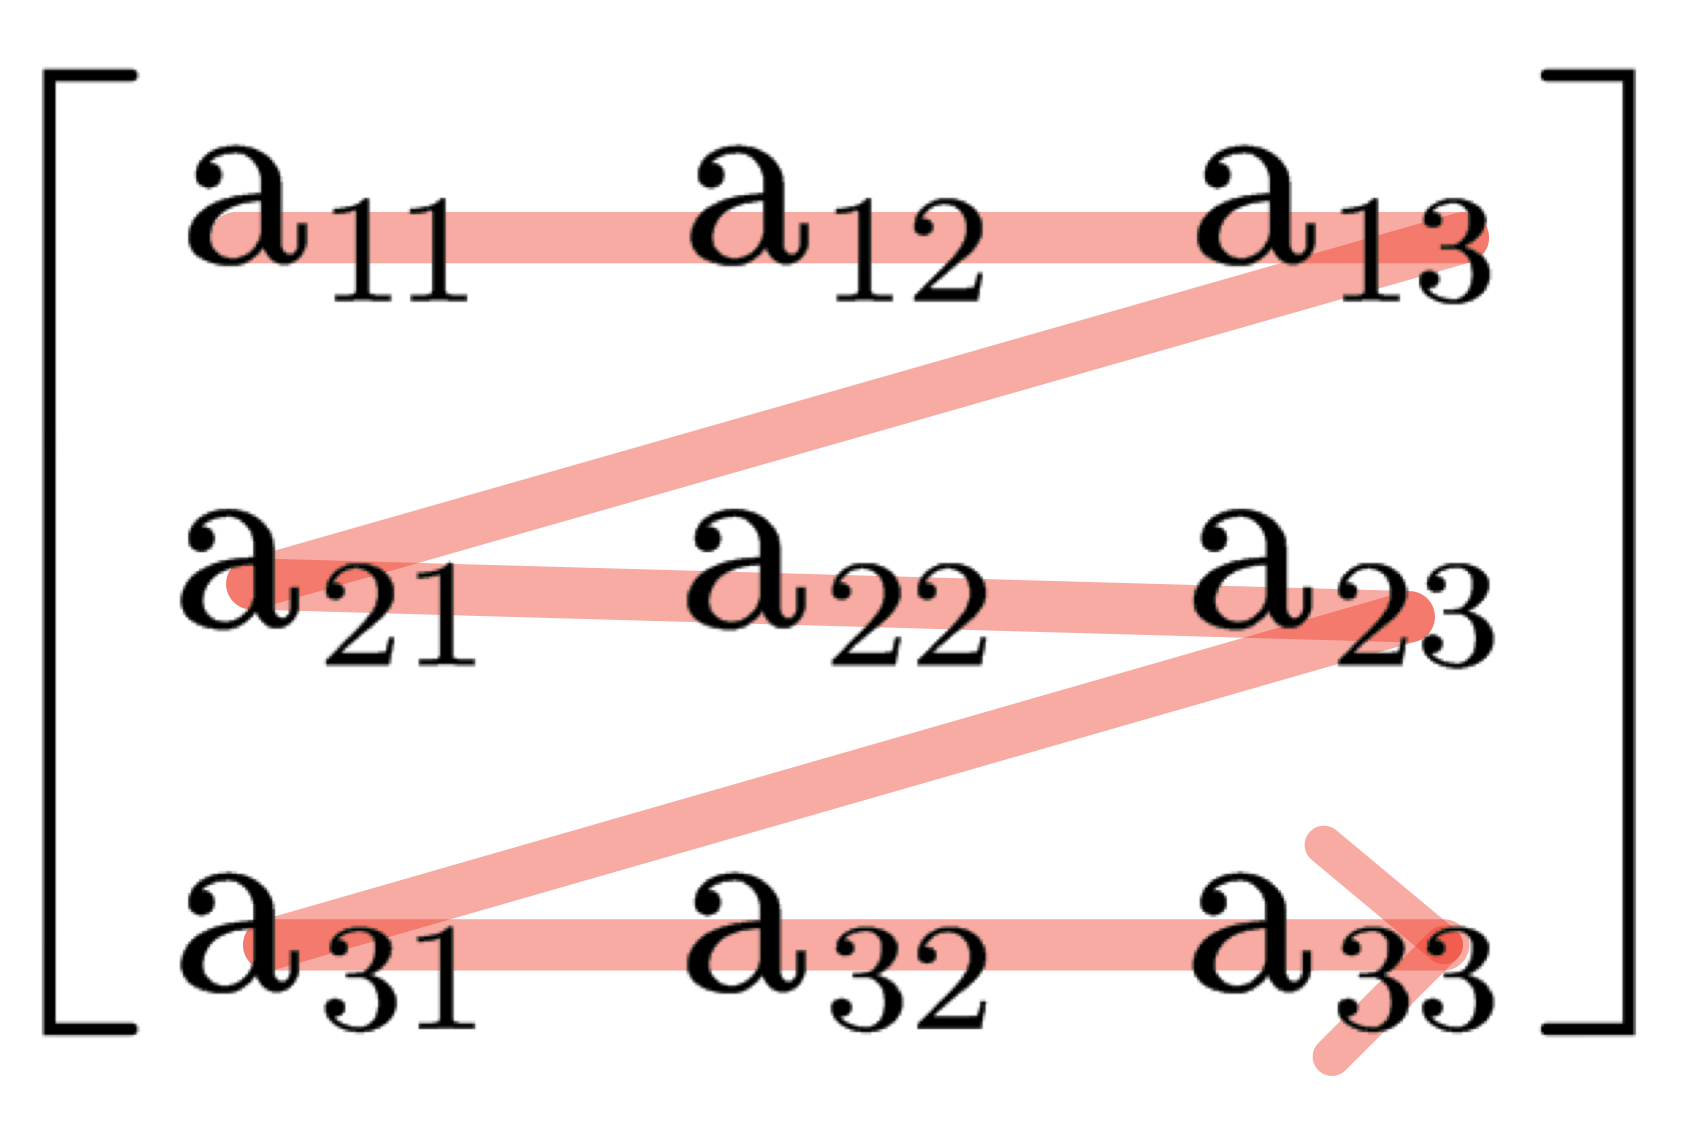
\includegraphics[width=0.5\textwidth]{rowmajor.png}
	\caption{CRS存储元素的顺序}
	\label{rowmajor}
\end{figure}

第三个向量JA是A中每个元素的列索引,同样针对稀疏矩阵T,我们利用CRS存储方式可以表示为:
\[
\begin{aligned}
A&=\left[ 1,3,4,2 \right] 
\\
IA&=\left[ 0,1,2,3,4 \right] 
\\
JA&=\left[ 2,0,3,0 \right] 
\end{aligned}
\]


\section{多项式拟合}
轨迹数据中的每条轨迹一般是由若干个点组成,有时需要通过这若干个点来拟合轨迹曲线,本文使用多项式来实现轨迹的拟合。
\subsection{理论基础}
在二维空间里,一条轨迹由n个点组成:$\left\{\left(x_{1}, y_{1}\right),\left(x_{2}, y_{2}\right), \dots,\left(x_{k}, y_{k}\right)\right\}$,若轨迹对应的函数为$f(x)$,多项式拟合则试图通过多项式来近似$f(x)$,n-1阶多项式的形式为$g\left( x \right) =a_0+a_1x+\cdots +a_{n-1}x^{n-1}$。

若通过n-1阶多项式来对n个坐标点对应的轨迹进行拟合,则将n个点的坐标带入n-1阶多项式可得到n个等式,将这n个等式通过矩阵表示则为:
\begin{equation}
\label{vandermonde}
\left[ \begin{matrix}
	1&		x_1&		\dots&		x_{1}^{n-1}\\
	1&		x_2&		\dots&		x_{2}^{n-1}\\
	\vdots&		\vdots&		\ddots&		\vdots\\
	1&		x_n&		\dots&		x_{n}^{n-1}\\
\end{matrix} \right] \left[ \begin{array}{c}
	a_0\\
	a_1\\
	\vdots\\
	a_{n-1}\\
\end{array} \right] =\left[ \begin{array}{c}
	y_1\\
	y_2\\
	\vdots\\
	y_n\\
\end{array} \right] 
\end{equation}

记$A=\left[ \begin{matrix}
	1&		x_1&		\dots&		x_{1}^{n-1}\\
	1&		x_2&		\dots&		x_{2}^{n-1}\\
	\vdots&		\vdots&		\ddots&		\vdots\\
	1&		x_n&		\dots&		x_{n}^{n-1}\\
\end{matrix} \right] $
,$\left|A^{T}\right|$则为范德蒙德行列式,故有:
\begin{equation}
\left|A^{T}\right|=\prod_{p>q}\left(x_{p}-x_{q}\right)
\end{equation}

若$x_0,x_1,…,x_n$彼此不相等,故此时存在唯一一个n-1次阶多项式能够包含所有数据点,此时用n-1阶多项式拟合的函数可以经过每一个点。

\subsection{麦克劳林级数及其收敛域}
若函数$f(x)$在$x_0$的某一个邻域内具有任意阶导数,则幂级数$\sum_{n=0}^{\infty}{\frac{f^{\left( n \right)}\left( x_0 \right)}{n!}}\left( x-x_0 \right) ^n$称为$f(x)$在$x_0$处的泰勒级数;当$x_0=0$时,此幂级数则称为麦克劳林级数,即$\sum_{n=0}^{\infty}{\frac{f^{\left( n \right)}\left( 0 \right)}{n!}}\left( x \right) ^n$。

假设$f(x)$在$x_0=0$处的麦克劳林级数收敛于$f(x)$,即当$n\rightarrow \infty $时,$f(x)$在$x_0=0$处的麦克劳林公式的余项$R_n(x)$对邻域中的点趋于0。此时,则有:
\begin{equation}
\label{maclaurin}
f\left( x \right) =\sum_{n=0}^{\infty}{\frac{f^{\left( n \right)}\left( 0 \right)}{n!}}\left( x \right) ^n
\end{equation}

等式\ref{maclaurin}右侧是幂级数,关于幂级数的收敛半径满足阿尔贝定理。

\textbf{阿贝尔定理}:如果幂级数$\sum_{n=0}^{\infty}{a_nx^n}$当$x=x_0(x_0 \ne 0)$时收敛,则对于一切满足$x<|x_0|$的x,幂级数$\sum_{n=0}^{\infty}{a_nx^n}$均绝对收敛;如果幂级数$\sum_{n=0}^{\infty}{a_nx^n}$在$x=x_1$处发散,则对于一切$x>|x_1|$的x,幂级数$\sum_{n=0}^{\infty}{a_nx^n}$均发散。

因此我们依据\ref{maclaurin}和阿贝尔定理可以得到函数$f(x)$其麦克劳林级数的收敛域。


\section{马尔科夫链理论}

\subsection{模型简介}

马尔可夫链,又称离散时间马可夫链\citing{norris1998markov},是一种离散状态空间的随机过程,其状态空间中的状态数是有限的,处于马尔科夫链中的状态会依据转移矩阵中对应的概率分布转移至其他状态或停留在同一状态,但每一次转移过程至于当下所处的状态有关,与当下状态之前所处的状态无关,这种特性称之为“马尔可夫性”,从中可以看出“马尔可夫性”是“无记忆”的。马尔科夫链是最常用的随机过程之一,依据“马尔可夫性”可以对现实生活中的很多模型进行建模,有着很广泛的应用场景。

已知满足马尔可夫性质的随机变量序列X1,X2,X3,...,依据马尔科夫性质的“无记忆性”有:
\begin{equation}
\label{markov_nature}
p\left(X_{n+1}=x | X_{1}=x_{1}, X_{2}=x_{2}, \ldots, X_{n}=x_{n}\right)=p\left(X_{n+1}=x | X_{n}=x_{n}\right)
\end{equation}

当转移概率与n无关时,则称此马尔科夫链是时齐马尔科夫链,本文后续提出的模型是建立在时齐马尔科夫链模型基础上构建的。时齐马尔科夫链满足:
\begin{equation}
\label{time_homogeneity}
p\left(X_{n+1}=x | X_{n}=y\right)=p\left(X_{n}=x | X_{n-1}=y\right)
\end{equation}

\subsubsection{随机游走}
随机游走是一种数学统计模型,它是一连串的轨迹所组成,其中每一次都是随机的。一种较常见的随机游走模型是在规则点阵上进行,称为点阵随机游走。在每一步中,标记的位置根据特定的概率分布从一点跳到另一个点。在简单点阵随机游走中,每一点只能跳到点阵中的相邻位置,形成点阵路径。

设定简单点阵随机游走是时齐的,其转移概率除了满足\ref{time_homogeneity},还满足:
\begin{equation}
\label{random_walk}
p_{ij}=p\left( X_{n+1}=i|X_n=j \right) =0 \left( i\notin Adj\left( j \right) \right) 
\\
\sum_{i\in Adj\left( j \right)}{p_{ij}=1}
\end{equation}

其中,Adj(j)表示点阵中与点j相邻的点的集合。

\section{本章小结}

本章对本文涉及到的理论技术进行了简要的概述。首先介绍了两种聚类算法:k-means算法和k-medoids算法,并通过伪代码展示了算法的流程,并分析了聚类算法的两种评估指标,即内部指标和外部指标;然后介绍了多项式拟合技术,引出了幂级数中关于收敛域的讨论;最后介绍了马尔科夫链模型,阐述了马尔科夫链建模的特性。本章介绍的所有理论技术对后文研究起到了举足轻重的作用。